% Full instructions available at:
% https://github.com/elauksap/focus-beamertheme

\documentclass{beamer}
\usetheme[numbering=progressbar]{focus}
\usepackage{tikz}
\usetikzlibrary{positioning}
\usetikzlibrary{shapes,arrows}
\usepackage{transparent}
\usepackage{fancyvrb}
\usepackage{listings}
\definecolor{main}{RGB}{47, 161, 219}
%\definecolor{textcolor}{RGB}{128, 128, 128}
\definecolor{background}{RGB}{240, 247, 255}
\definecolor{textcolor}{RGB}{85, 87, 83}
\title{D4 Project}
\subtitle{PIBS - Passive Identification of BackScatter}
\author{TEAM CIRCL}
\titlegraphic{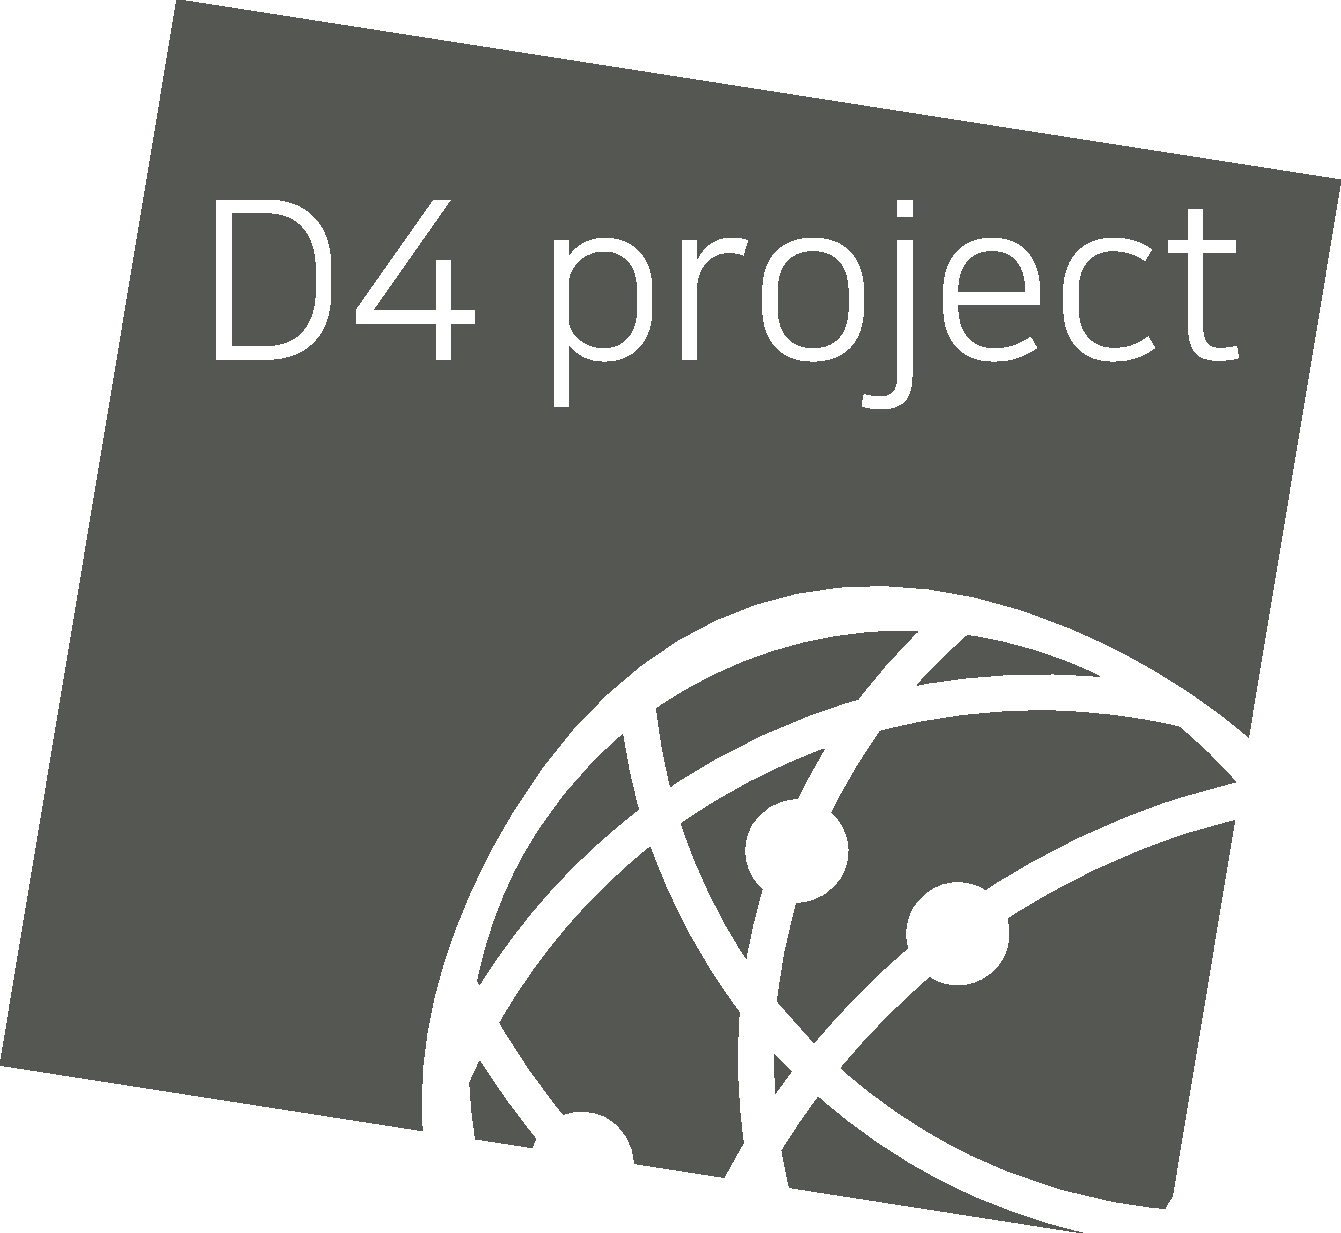
\includegraphics[scale=0.20]{d4-logo.pdf}}
\institute{Team CIRCL \\ \url{https://www.d4-project.org/}}
\date{20190329}

\begin{document}
    \begin{frame}
        \maketitle
    \end{frame}


\begin{frame}
    \frametitle{Open problems}
    \framesubtitle{Filter out potential backscatter traffic}
    \begin{itemize}
        \item Differentiate Scanning activities\footnote{\url{https://nmap.org/book/man-port-scanning-techniques.html}}
        \begin{itemize}
            \item TCP SYN scan
            \item XMAS scans
            \item ACK scans
            \item TCP Window scan
            \item TCP Maimon scan
            \item Custom TCP scan
        \end{itemize}
        \item Misconfigured systems
        \item Malicious packets against D4 infrastructure
	\item Handling file rotations
	\item Expiration of state tables
    \end{itemize}
\end{frame}


\begin{frame}[fragile]
    \frametitle{Handling TCP SYN scans}
    \begin{itemize}
        \item Was the IP seen before?
        \item Keep a hash table of all encountered IP addresses
        \item Consider only IP addresses where the TCP SYN flag is set
        \item Insert the IP and the timestamp in the hash table
        \item Display new IP addresses
    \end{itemize}
    \begin{block}{PIBS tool}
        \begin{verbatim}
            pibs -r pcapfile.cap -b
        \end{verbatim}
    \end{block}
\end{frame}

\begin{frame}
    \frametitle{Using PIBS as D4 analyzer}
    \begin{itemize}
        \item Chaining PIBS to D4 server
        \item PIBS polls a redis queue for new created files
        \item Each PIBS instance can have its UUID
    \end{itemize}
    \begin{block}{PIBS tool}
        pibs -u e344c4fb-442e-45a6-92b9-d8e30aeef448 -z 127.0.0.1 -p 6379 -y 2
    \end{block}
    \begin{itemize}
        \item -u specifies uuid
        \item -z specifies the redis server
        \item -p specifies the port of the redis server
        \item -y specifies the redis database
    \end{itemize}
\end{frame}

\begin{frame}
    \frametitle{Using PIBS for further exploration}
    \begin{itemize}
        \item Often it is unknown which fields should be analysed during refinement
        \item Read raw pcap and output raw pcap
        \item Output pcap file can be further investigated with other tools such as Wireshark
    \end{itemize}
    \begin{block}{PIBS tool}
        pibs -r source.cap.gz -w backscatter.cap
    \end{block}
\end{frame}
\end{document}
